\section*{Aspectos Técnicos de la Convocatoria}
La subestación Huila 230 kV contará con una configuración tipo interruptor y medio, incluyendo cuatro bahías de línea y dos bahías de transformación, todas con cortes centrales. Se establecerán dos diámetros completos y dos incompletos a 230 kV, garantizando alta confiabilidad operativa y posibilidad de expansión futura mediante enlaces removibles. La subestación podrá ser de tipo convencional (AIS), aislada en gas (GIS) o una solución híbrida, según normativa aplicable. Tendrá niveles de aislamiento de 1050 kV para el impulso tipo rayo y 460 kV a frecuencia industrial. Además, dispondrá de servicios auxiliares en AC (120/208 V, tres fases, cuatro hilos) y DC (125 V).

El sistema eléctrico del proyecto operará con una tensión nominal de 230 kV, una frecuencia asignada de 60 Hz, con puesta a tierra sólida y un número de fases igual a tres (3), cumpliendo así con los estándares técnicos requeridos para el sistema de transmisión en alta tensión. Deben garantizarse sistemas de control, protecciones, medición, comunicaciones e infraestructura asociada, compatibles con la infraestructura existente.

Las líneas de transmisión del proyecto operarán a una tensión nominal de 230 kV e implican la construcción de una línea de doble circuito o dos líneas independientes desde la subestación Huila: aproximadamente 6 km hacia la línea Betania–Mirolindo, para su reconfiguración como Betania–Huila–Mirolindo, y 6 km hacia la línea Betania–Tuluní, para conformar Betania–Huila–Tuluní. El proyecto incluye las adecuaciones y conexiones necesarias para integrar las nuevas líneas con las existentes. Las líneas serán preferentemente aéreas, utilizando torres auto soportadas, postes, estructuras compactas y/o tramos subterráneos, con estructuras de soporte diseñadas para doble circuito o circuito sencillo, y la posibilidad de compartir infraestructura existente.
\section*{Aspectos de Diseño de la Convocatoria}

Todos los tramos de línea deberán contar con uno o dos cables de guarda (convencionales u OPGW). En líneas nuevas, al menos uno de estos debe ser tipo OPGW. En los tramos que reconfiguren líneas existentes, los cables de guarda que se instalen deberán tener características técnicas iguales o superiores a los de la línea existente.

La altura sobre el nivel del mar (asociada a estimativos preliminares) está comprendida entre los 440 m y 490 m para la reconfiguración de la línea Betania - Huila - Mirolindo 230 kV y Betania - Huila - Tuluní 230 kV. Sin embargo, tanto la longitud real como la altura real sobre el nivel del mar serán función del trazado, diseño y estudios pertinentes que debe realizar el inversionista seleccionado.

El transmisor debe determinar en su diseño los materiales que utilizará en la ejecución de las puestas a tierra de las estructuras de la línea, teniendo en cuenta la vida útil, la frecuencia de las inspecciones y mantenimientos, la posibilidad del robo de los elementos de cobre, así como la corrosividad de los suelos en el sitio de cada torre.

Para el diseño de las líneas de transmisión, se establecieron criterios técnicos que garantizan un desempeño seguro y eficiente. Los conductores de fase deben soportar una capacidad mínima de 1000 A y tener una resistencia máxima de 0,030 ohmios/km a 20 °C. Además, se consideran condiciones térmicas, mecánicas y ambientales, asegurando el cumplimiento con normas técnicas y la confiabilidad en la operación del sistema.

En cuanto a los niveles máximos de radiointerferencia, se exige una relación señal-ruido mínima de 22 dB a 1000 kHz, medida a 80 metros del eje de la línea en zonas rurales y a 40 metros en zonas urbanas, bajo condiciones de buen tiempo.


\subsection*{Esquema unifilar y diagrama esquemático}

\begin{figure}[h!] % 'h' coloca la figura aquí
    \centering % Centra la imagen
    \begin{subfigure}{0.5\textwidth}
        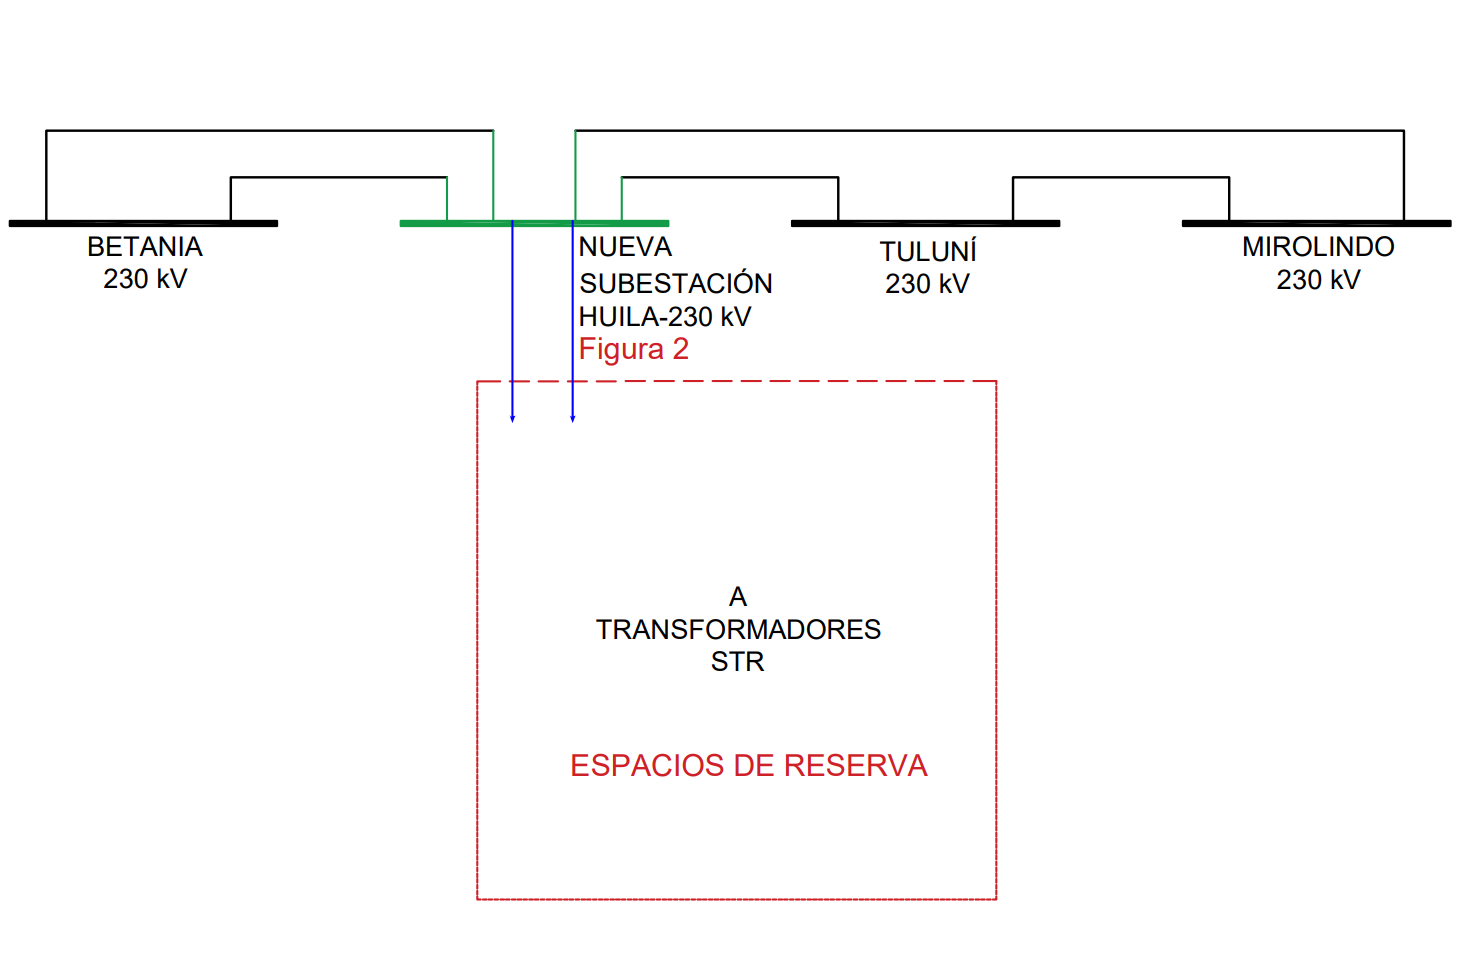
\includegraphics[width=1\textwidth]{1mer avance foticos/Esquema unifilar diagrama esquemático.png}
        \caption{en la figura del diagrama unifilar esquemático como\\ se evidenciará mas adelante en el trazado de la ruta se \\conectará la nueva subestación Huila de dicha forma.} % Título de la figura
        \label{fig:Esquema} % Etiqueta para referencias
    \end{subfigure}
    \hfill % Espacio horizontal entre las subfiguras
    \begin{subfigure}{0.5\textwidth}
        \centering % Centra la imagen
        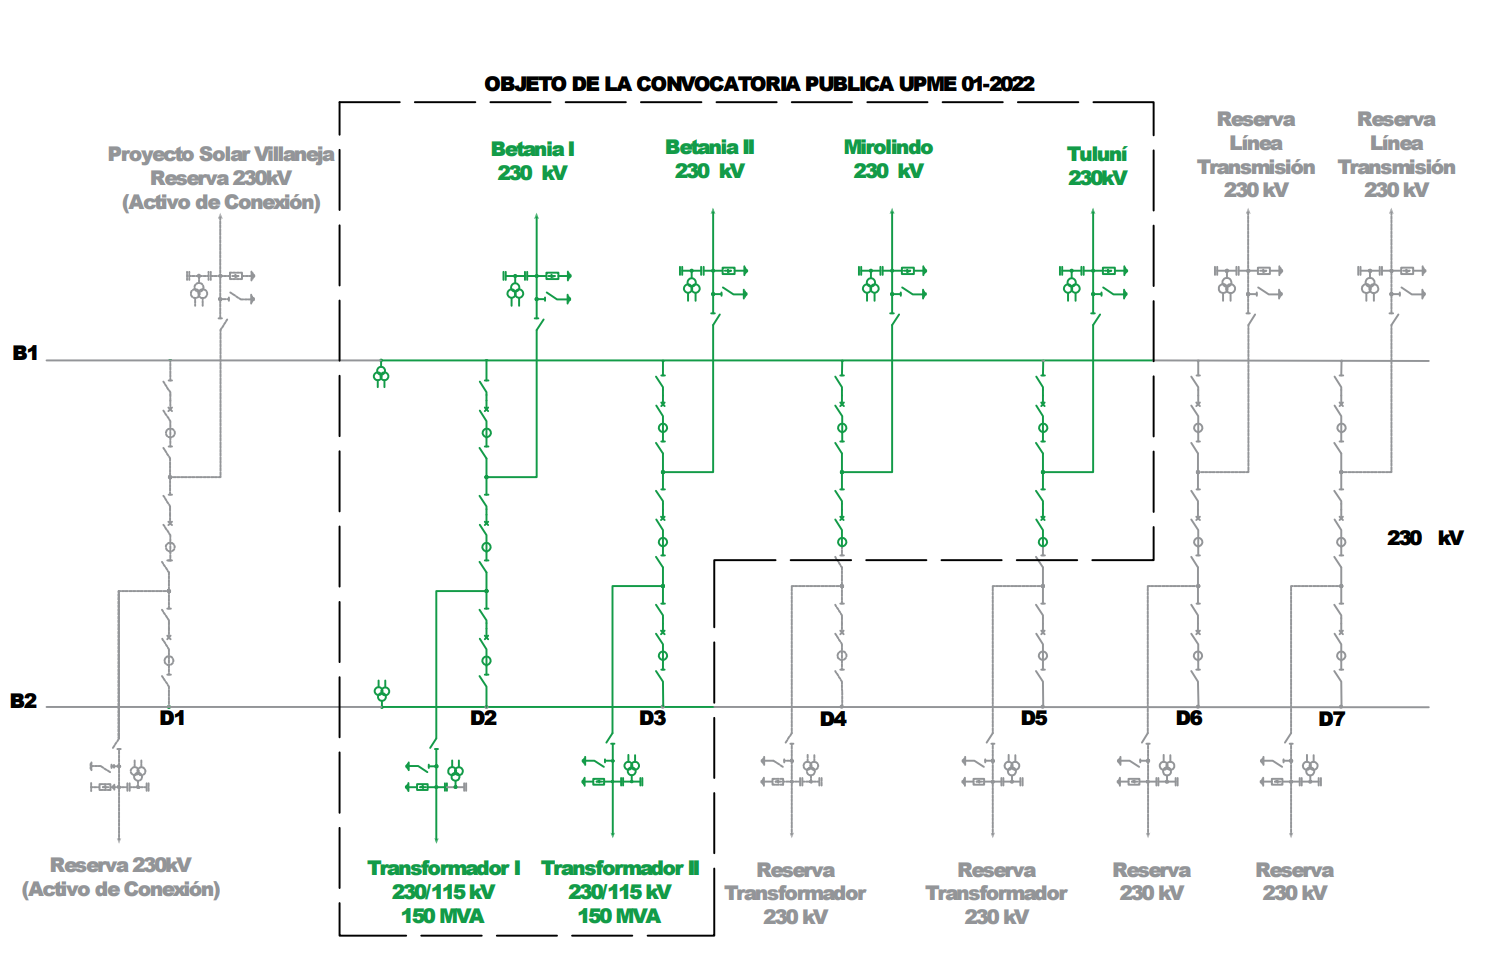
\includegraphics[width=1\textwidth]{1mer avance foticos/Esquema unifilar de la subestación huila 230kv.png}
        \caption{Esquema unifilar de la subestación huila 230kv.} % Título de la figura
        \label{fig:unifilar} % Etiqueta para referencias
    \end{subfigure}
    \label{fig:dos-imagenes}
\end{figure}



%En la \figurename~\ref{fig:unifilar} se muestra un ejemplo de cómo insertar y referenciar imágenes en LaTeX. Este formato permite que, si la imagen se mueve a otra parte del documento, la referencia se actualice automáticamente.

